% this file is called up by thesis.tex
% content in this file will be fed into the main document

\chapter{Designing a RDMA Key Value store}\label{ch:design} % top level followed by section, subsection


% ----------------------- paths to graphics ------------------------

% change according to folder and file names
\ifpdf
    \graphicspath{{7/figures/PNG/}{7/figures/PDF/}{7/figures/}}
\else
    \graphicspath{{7/figures/EPS/}{7/figures/}}
\fi


% ----------------------- contents from here ------------------------
In this section, the design of the used key value store is shown, along with design decision made for RDMA.
Further, benchmarking strategy will be explained, used to evaluate the performance of various RDMA transport types.
Lastly, an overview of DAS-5 is given, which will be used to run benchmarks.
This can be used when comparisons are made with other findings.

\section{Key value store}
This thesis is focused on the scalability using RDMA, and will not focus on advancing KV-stores.
Therefore, a trivial KV store has been used.
For this KV store, \textit{SET} and \textit{GET} instructions are mainly used, a long with other commands for testing purposes.
All possible commands can be seen in figure \ref{fig:method}.

\subsection{Requests}

\begin{figure}
    \centering
    \subfigure[Request structure] {
        \centering
        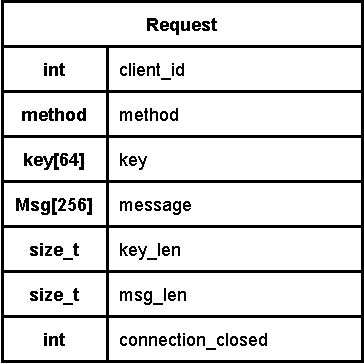
\includegraphics[height=6cm]{figures/PDF/request}
        \label{fig:request}
    }
    \subfigure[Values for method] {
        \centering
        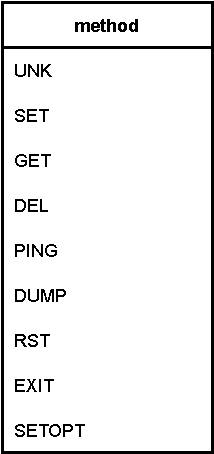
\includegraphics[height=6cm]{figures/PDF/method}
        \label{fig:method}
    }
    \caption{Structure for request with accommodated method}
\end{figure}

For a client to interact with a KV server, the client has to send a request towards the server.
A request is structured as shown in figure \ref{fig:request}.
This key is used to identify the correct index within the hash table.
A field for payload is always sent, however only used for \textit{SET} commands.
This is to have a constant data size, key having 64 bytes and message 256.

\subsection{Response}

\begin{figure}
    \centering
    \subfigure[Response structure] {
        \centering
        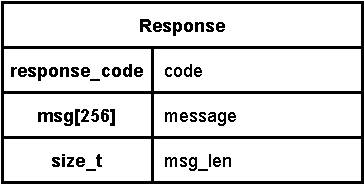
\includegraphics{figures/PDF/response}
        \label{fig:response}
    }
    \subfigure[Respond codes] {
        \centering
        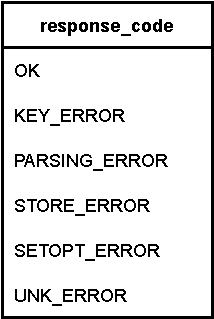
\includegraphics[height=5cm]{figures/PDF/response_code}
        \label{fig:codes}
    }
    \caption{Structure for response with accommodated response codes}
\end{figure}

After processing a request the server will always send an respond.
The structure of which is shown in \ref{fig:response}.
In case of a successful execution, an \textit{OK} code will be given.
For \textit{GET} requests a payload is given along with this \textit{OK} code, this is the value requested.
Upon error, an error code will be sent back: \textit{PARSING\_ERROR}, or \textit{UNKNOWN (UNK)}, latter of which is when the given command is unknown.
Other response codes can be seen in \ref{fig:codes}


\subsection{Hash table}

\begin{figure}
    \centering
    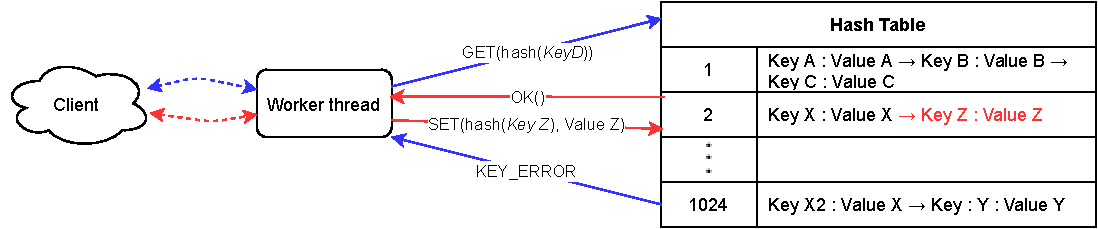
\includegraphics[width=\columnwidth]{figures/PDF/Client_to_hash_table}
    \caption[Key value server layout]{Key value server layout. Process worker thread takes with incoming requests, and what response is sent. A successful \textit{SET} request is shown in red, adding a value "Value Z" to the internal linked list, with key "Key Z". Blue is an unsuccessful \textit{GET} where the key is not known.}
    \label{fig:hash_table}
\end{figure}

Internally, a hash table with 1024 buckets is used.
Each bucket contains a linked list of key-value pairs.
Figure \ref{fig:hash_table} shows the structure of the KV store used.
It should be noted, a linked list approach, as used here, does not scale well.
As buckets are filled, either due to a hash collisions or extensive use, \textit{GET} requests can cause for significantly delay, especially when encountering a key miss.
This can be partially solved with a large hash table, this however will not be a long term solution, along with strong hash function.
However, with a 95\% GET request workload, the scalability issues will not show a significant performance loss.
More over, in section \ref{sec:benchmark-design} this issue will be kept constant throughout experiments.

\subsection{Multithreaded}\label{subsec:multithreaded}
The KV server implemented for this thesis is also multithreaded.
For every client a worker thread process will be created.
This thread will read requests, process accordingly, and send back a response, all the while the main thread is used to accept and set up for new clients.
In this way, worker threads are unaffected by new clients that are connecting.

To ensure concurrent and correct operation, each bucket has a mutex lock, and each key-value pair a read-write lock.
This could cause performance loss as been seen in FaSST \cite{kalia2016fasst, qiu2018toward}.

\section{RDMA}\label{sec:rdma2}
For this research, the two-sided verbs \textit{SEND} and \textit{RECV} are used for RDMA.
Looking at table \ref{tab:transport-verb}, across all transportation types \textit{SEND}/\textit{RECV} is the only available verb.
This might come at a cost of performance, due to the channel schematic and minor CPU involvement.
It has been shown that in some use cases, one-sided \textit{WRITE} operations performs superior compared to \textit{SEND}\cite{kalia2014using}.
However, this difference is minimal, and the use of \textit{WRITE} is not possible for this research.

To establish a baseline improvement and scalability, no optimizations are implemented.
In section \ref{ch:future-improvements} possible optimizations are discussed.

\subsection{Queue pairs}
Connection based QP's will be handled similarly as in section \ref{subsec:multithreaded} above.
Every worker thread will have a client connected QP, which can only communicate with this client.
This differs for UD.
As stated in section \ref{sec:rdma}, any UD QP can communicate with any other UD QP.
This meaning, that the server only needs one QP for all clients.
A worker thread is still created for every client, however, in the case of UD, all threads use a shared queue.

%TODO ADD MORE GRAPHICS


\section{Benchmark design}\label{sec:benchmark-design}
To evaluate the performance and scalability of the RDMA KV store, a multiclient benchmark has been made.
In total, 10 million tasks will be divided among clients.
This number is constant to lessen the scalability issues with the underlying hash table.
A task involves two operations, sending a request and receiving response.
Only once a response is received from the server, can the client continue to the next task.
This meaning that the full potential of RDMA is not being used, however it has been chosen for correctness, and such that latency can be evaluated accurately on a per-task level. %TODO MAYBE I SHOULD CONTINUE?

During client benchmark execution, the time will be taken at two points: before sending request, and after receiving response.
With this, the throughput and latency of every client and every operation can be traced back.
Time will be gathered with the $gettimeofday$ function, and as accuracy achieves measurements at $\mu$sec scale.
These times will be kept in an array, and be returned after completing its tasks.
The time will be later written to CSV files perform statistical analysis and graphs are drawn, as can be seen later on in the evaluation section \ref{ch:evaluation}.
For this, Python 3.6\cite{python} is used, along with pandas\cite{pandas} and matplotlib\cite{matplotlib}.

The benchmark is designed to evaluate each transportation types under similar conditions, and will follow the same path.
Once a client is setup and connected with the server, it will start performing its tasks.
These tasks follow the 30:1 \textit{GET}/\textit{SET} ratio that found by Atikoglu et. al.\cite{atikoglu2012workload}.
A \textit{SET} request has a 5\% chance of being generated.
This is done by generating a random number as follows: $rand() \bmod 100 <= 5$.
Else a \textit{GET} request is generated.
The client sends out the request, and waits for response.

\subsection{Experimental Setup}\label{subsec:experimental-setup}
All performance tests and results have been gathered on the DAS-5 computing cluster\cite{das5}.
This distributed system of computers spread across the Netherlands, and is used by research groups from VU Amsterdam, TU Delft, Leiden University, and many more.
Each cluster varies slightly in specifications, however each, is equipped with dual Intel E5-2630v3 8-core CPUs, a 56 Gbit/s Inifiniband (IB) RDMA networking, and 1 Gbit/s classical ethernet networking.
The specifications of each cluster is as shown in table \ref{tab:das5}.

All experiments make use of the IB network card, and is also configured to run TCP/IP.
Furthermore, at least two nodes are used, his ensures that the server and clients are separated.

\begin{table}
    \centering
    \begin{tabular}{lrlllll}
        \toprule
        \textbf{Cluster} & \textbf{Nodes} & \textbf{CPU type} & \textbf{Frequency (GHz)} & \textbf{Memory (GB)} & \textbf{Network} \\
        \midrule
        VU & 68 & dual 8-core & 2.4 & 64 & IB and GbE \\
        LU & 24 & dual 8-core & 2.4 & 64 & IB and GbE \\
        UvA & 18 & dual 8-core & 2.4 & 64 & IB and GbE \\
        TUD & 48 & dual 8-core & 2.4 & 64 & IB and GbE \\
        UvA-MN & 31 & dual 8-core & 2.4 & 64 & IB and GbE \\
        ASTRON & 9 & dual 8/10/14-core & 2.6 & 128/512 & IB, 40 GbE, GbE \\
        \bottomrule
    \end{tabular}
    \caption{DAS-5 cluster specifications}
    \label{tab:das5}
\end{table}






% ---------------------------------------------------------------------------
% ----------------------- end of thesis sub-document ------------------------
% ---------------------------------------------------------------------------